\documentclass{beamer}
\usetheme{Madrid}
\usepackage{tikz}
\usetikzlibrary{shapes}

%\tikzstyle{class-name} =[definition_list]
\tikzstyle{startstop} = [ellipse, draw]
\tikzstyle{normal} = [rectangle, draw, text centered]
\tikzstyle{decision} = [diamond, aspect = 4, draw]
\tikzstyle{inputoutput} = [trapezium, trapezium left angle = 70, trapezium right angle = 110, draw]


\title[beamer class]{Practice on Beamer and Tikz}
\author[muntaka]{Muntaka Ibnath}
\institute[BUET]{Bangladesh University of Engineering and Technology}
\date{\today}



\begin{document}
	\frame{\titlepage}
	\begin{frame}
		\frametitle{Introduction to Beamer}
		\begin{itemize}
			\item Beamer is very important for technical presentation.
			
		\end{itemize}
	\end{frame}

	\begin{frame}
		\frametitle{Columns}
		\begin{columns}
			\column{0.2\textwidth}
			Tikz is an important tool for creating self-generated figures.
			$ E=mc^2 $
			\column{0.2\textwidth}
			Today we will cover both beamer and tikz.
		\end{columns}
	\end{frame}

	\begin{frame}
		\begin{alertblock}{Block Header}
			Here are some text inside block.
		\end{alertblock}
	\end{frame}

	\begin{frame}
		\begin{figure}[h]
			\centering
			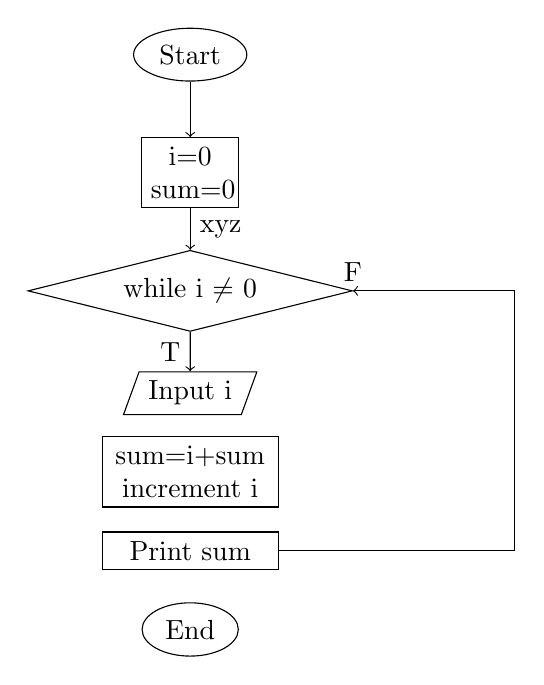
\begin{tikzpicture}
				%\node[class-name,position_info,text width=,](unique-id){Text Inside};
				\node[startstop](start) {Start};
				\node[normal, below of=start, text width = 1 cm,yshift=-0.5cm](i_sum) {i=0  sum=0};
				\node[decision,below of=i_sum,yshift=-0.5cm](while) {while i $ \neq $ 0};
				\node[inputoutput,below of=while,yshift=-0.3cm](input) {Input i};
				\node[normal,below of=input,text width=2cm](sum_incr) {sum=i+sum increment i};
				\node[normal,below of=sum_incr,text width=2cm](print) {Print sum};
				\node[startstop,below of=print](end) {End};
				
				%\draw[] (n1 id) -- (n2 id) ;
				\draw[->] (start) -- (i_sum);
				\draw[->] (i_sum) -- node[right]{xyz}(while);
				\draw[->] (while) -- node[left] {T} (input);
				\draw[->] (print.east) -- ++(3,0) |- (while.east)node[above] {F};
			\end{tikzpicture}
			\caption{LIWC Categories}
		\end{figure}
	\end{frame}

	
\end{document}

